\documentclass{beamer}

\mode<presentation> {

% The Beamer class comes with a number of default slide themes
% which change the colors and layouts of slides. Below this is a list
% of all the themes, uncomment each in turn to see what they look like.

%\usetheme{default}
%\usetheme{AnnArbor}
%\usetheme{Antibes}
%\usetheme{Bergen}
%\usetheme{Berkeley}
%\usetheme{Berlin}
%\usetheme{Boadilla}
%\usetheme{CambridgeUS}
%\usetheme{Copenhagen}
%\usetheme{Darmstadt}
%\usetheme{Dresden}
%\usetheme{Frankfurt}
%\usetheme{Goettingen}
%\usetheme{Hannover}
%\usetheme{Ilmenau}
%\usetheme{JuanLesPins}
%\usetheme{Luebeck}
\usetheme{Madrid}
%\usetheme{Malmoe}
%\usetheme{Marburg}
%\usetheme{Montpellier}
%\usetheme{PaloAlto}
%\usetheme{Pittsburgh}
%\usetheme{Rochester}
%\usetheme{Singapore}
%\usetheme{Szeged}
%\usetheme{Warsaw}

% As well as themes, the Beamer class has a number of color themes
% for any slide theme. Uncomment each of these in turn to see how it
% changes the colors of your current slide theme.

%\usecolortheme{albatross}
%\usecolortheme{beaver}
%\usecolortheme{beetle}
%\usecolortheme{crane}
%\usecolortheme{dolphin}
%\usecolortheme{dove}
%\usecolortheme{fly}
%\usecolortheme{lily}
%\usecolortheme{orchid}
%\usecolortheme{rose}
%\usecolortheme{seagull}
%\usecolortheme{seahorse}
%\usecolortheme{whale}
%\usecolortheme{wolverine}

%\setbeamertemplate{footline} % To remove the footer line in all slides uncomment this line
%\setbeamertemplate{footline}[page number] % To replace the footer line in all slides with a simple slide count uncomment this line

%\setbeamertemplate{navigation symbols}{} % To remove the navigation symbols from the bottom of all slides uncomment this line
}

\usepackage{graphicx} % Allows including images
\usepackage{booktabs} % Allows the use of \toprule, \midrule and \bottomrule in tables
\usepackage[utf8]{inputenc}

%----------------------------------------------------------------------------------------
%	TITLE PAGE
%----------------------------------------------------------------------------------------

\title[Google Home]{Google Home Midterm Presentation} % The short title appears at the bottom of every slide, the full title is only on the title page

\author{Mehmet Kardan, Hanna Köb, Mathias Meinschad, Daniel Linter} % Your name
\institute[UCLA] % Your institution as it will appear on the bottom of every slide, may be shorthand to save space
{
University of Innsbruck - SIT \\ % Your institution for the title page
}
\date{\today} % Date, can be changed to a custom date

\begin{document}

\begin{frame}
\titlepage % Print the title page as the first slide
\end{frame}

\begin{frame}
\frametitle{Overview} % Table of contents slide, comment this block out to remove it
\tableofcontents % Throughout your presentation, if you choose to use \section{} and \subsection{} commands, these will automatically be printed on this slide as an overview of your presentation
\end{frame}

%----------------------------------------------------------------------------------------
%	PRESENTATION SLIDES
%----------------------------------------------------------------------------------------

%------------------------------------------------
\section{Overview}

\begin{frame}
\frametitle{Overview}
\begin{center}

\includegraphics[scale=0.35]{pictures/google-home.png} 
\end{center}
\begin{itemize}
\item Founded by Google in 2016
\item Development through Googles developer console and Dialogflow
\item Creating skills pretty easy
\item No programming skills required
\end{itemize}
\end{frame}

%------------------------------------------------

\section{Execution Path}

\begin{frame}
\frametitle{Execution Path}
\begin{center}
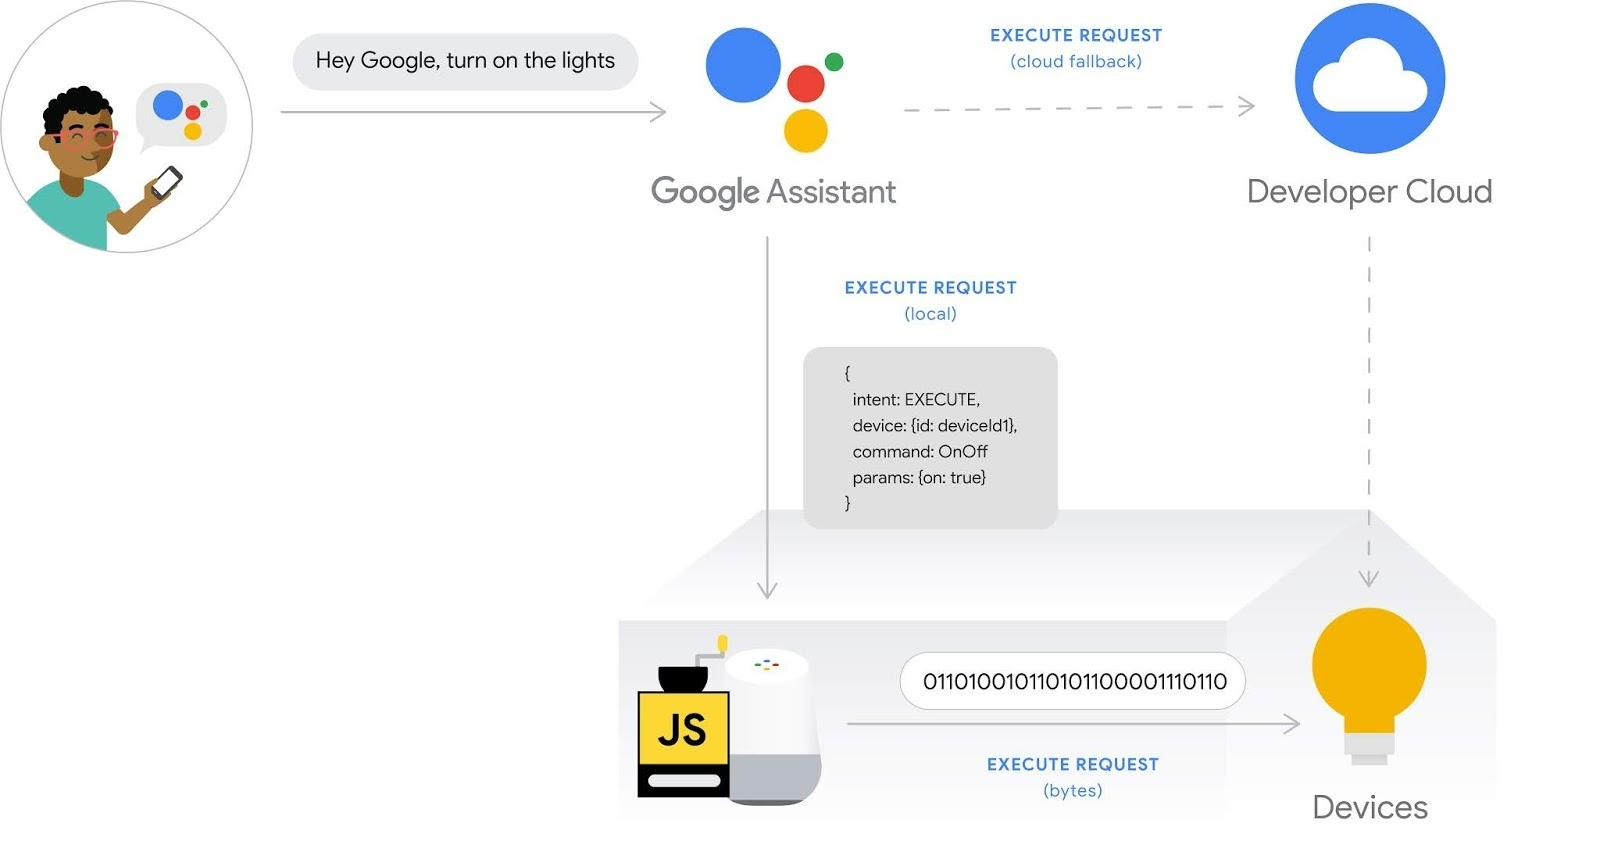
\includegraphics[scale=0.2]{pictures/execution-path.png}
\end{center}
\end{frame}

%------------------------------------------------

\section{Developer Console}

\begin{frame}
\frametitle{Developer Console}
\begin{center}
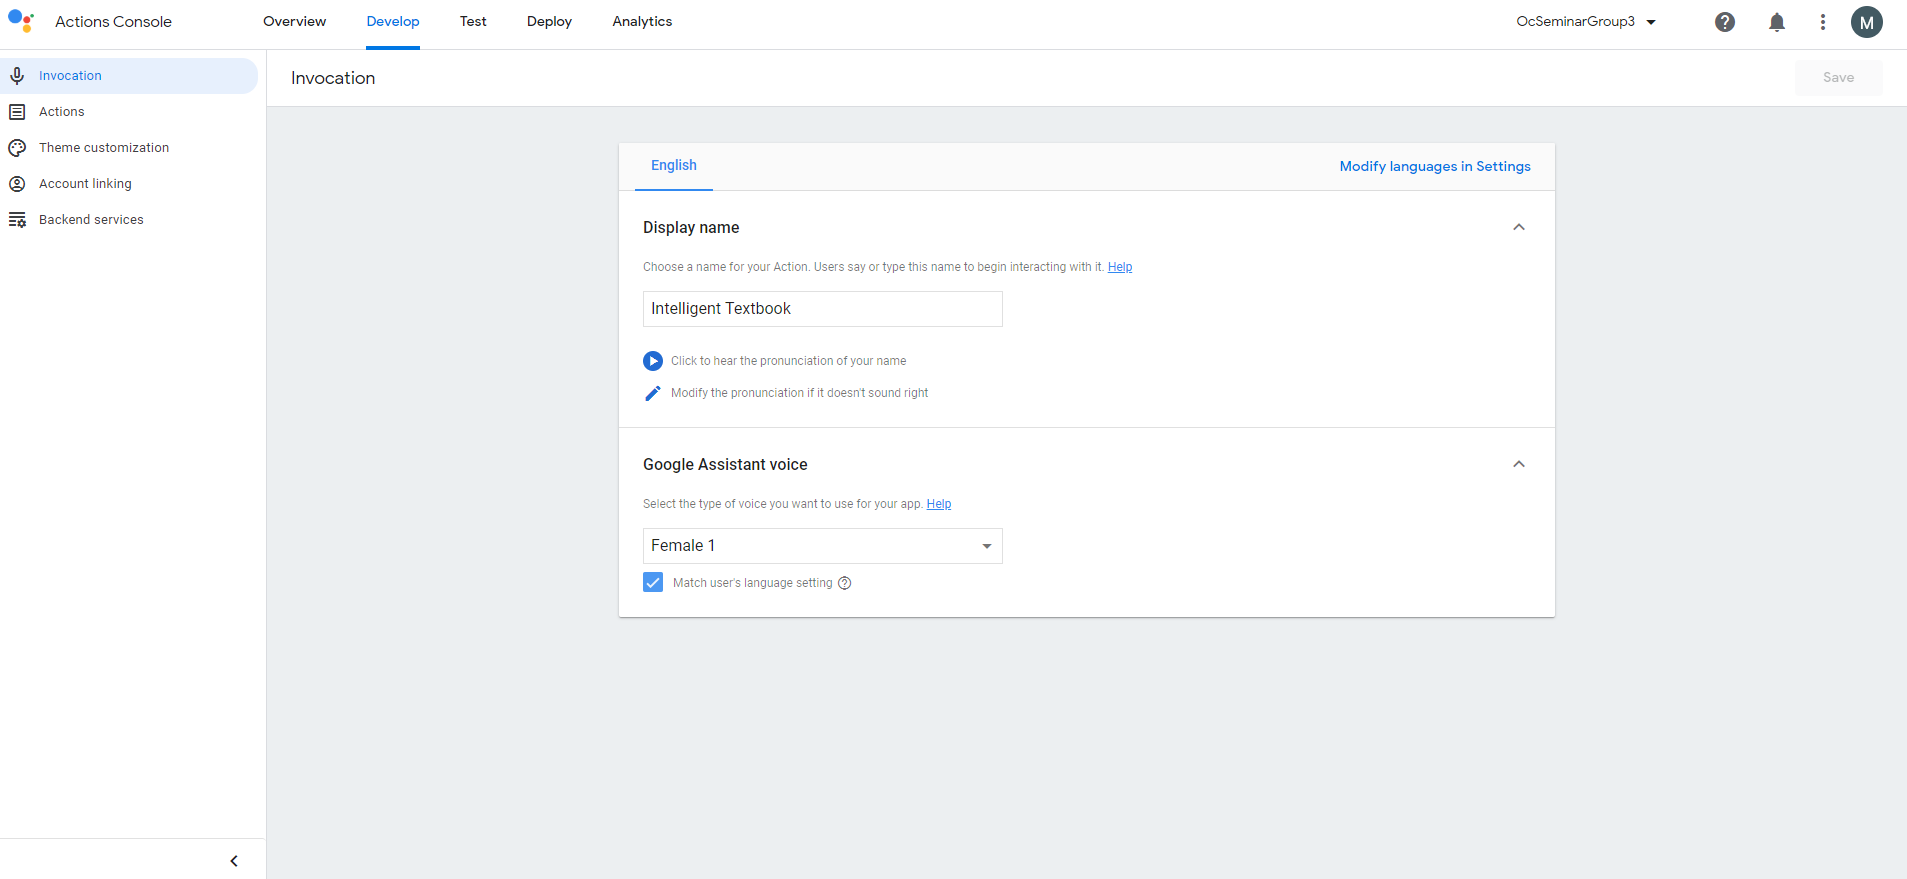
\includegraphics[scale=0.23]{pictures/developer-console.png}
\end{center}
\end{frame}

\begin{frame}
\frametitle{Developer Console cont'd}
\begin{center}
\begin{itemize}
\item Gives an overview of your skill
\item Specifies general settings
\item Gives the user the ability to test their skill
\item Deployment of the skill
\end{itemize}
\end{center}
\end{frame}

%------------------------------------------------

\section{Dialogflow}

\begin{frame}
\frametitle{Dialogflow}
\begin{center}
\begin{itemize}
\item Service developed and provided by Google
\item Natural language tool to create conversational user interfaces for apps, chatbots, etc.
\item By adding 'Training phrases' Dialogflow automatically trains the machine learning model
\end{itemize}
\end{center}
\end{frame}


%------------------------------------------------


\begin{frame}
\frametitle{Dialogflow cont'd}
\begin{block}{Concepts}
\begin{itemize}
\item Intents
\begin{itemize}
\item Each intent describes an intent a user might have
\item E.g. check prices, get opening hours or book a repair
\item By communicating with the interface, Dialogflow classifies the user's intent and performs the associated action
\item An intent can require some parameters such as a date in order to book a repair
\end{itemize}
\item Entities
\begin{itemize}
\item Each intent parameter has a type and therefore belongs to an entity
\item There are predefined system entities for dates, colors, addresses, etc.
\item Define entities to make Dialogflow 'understand' your vocabulary
\item E.g. Entity 'bike-type' with the instances road bike and mountain bike
\end{itemize}
\item Knowledge Base
\begin{itemize}
\item Complement defined intents
\item Used to find automated responses
\end{itemize}
\end{itemize}
\end{block}
\end{frame}


%------------------------------------------------

\subsection{Intents}

\begin{frame}
\frametitle{Intents}
\begin{center}
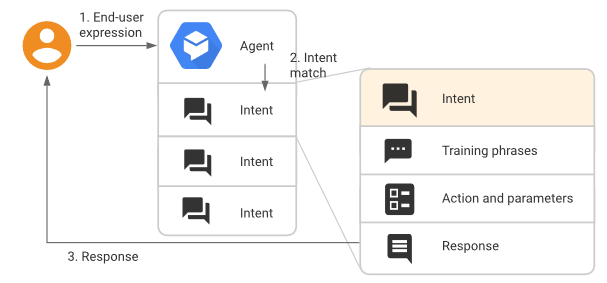
\includegraphics[width=0.8\textwidth]{pictures/intent.png}

\end{center}
\end{frame}

\begin{frame}
\frametitle{Intents cont'd}
\begin{center}
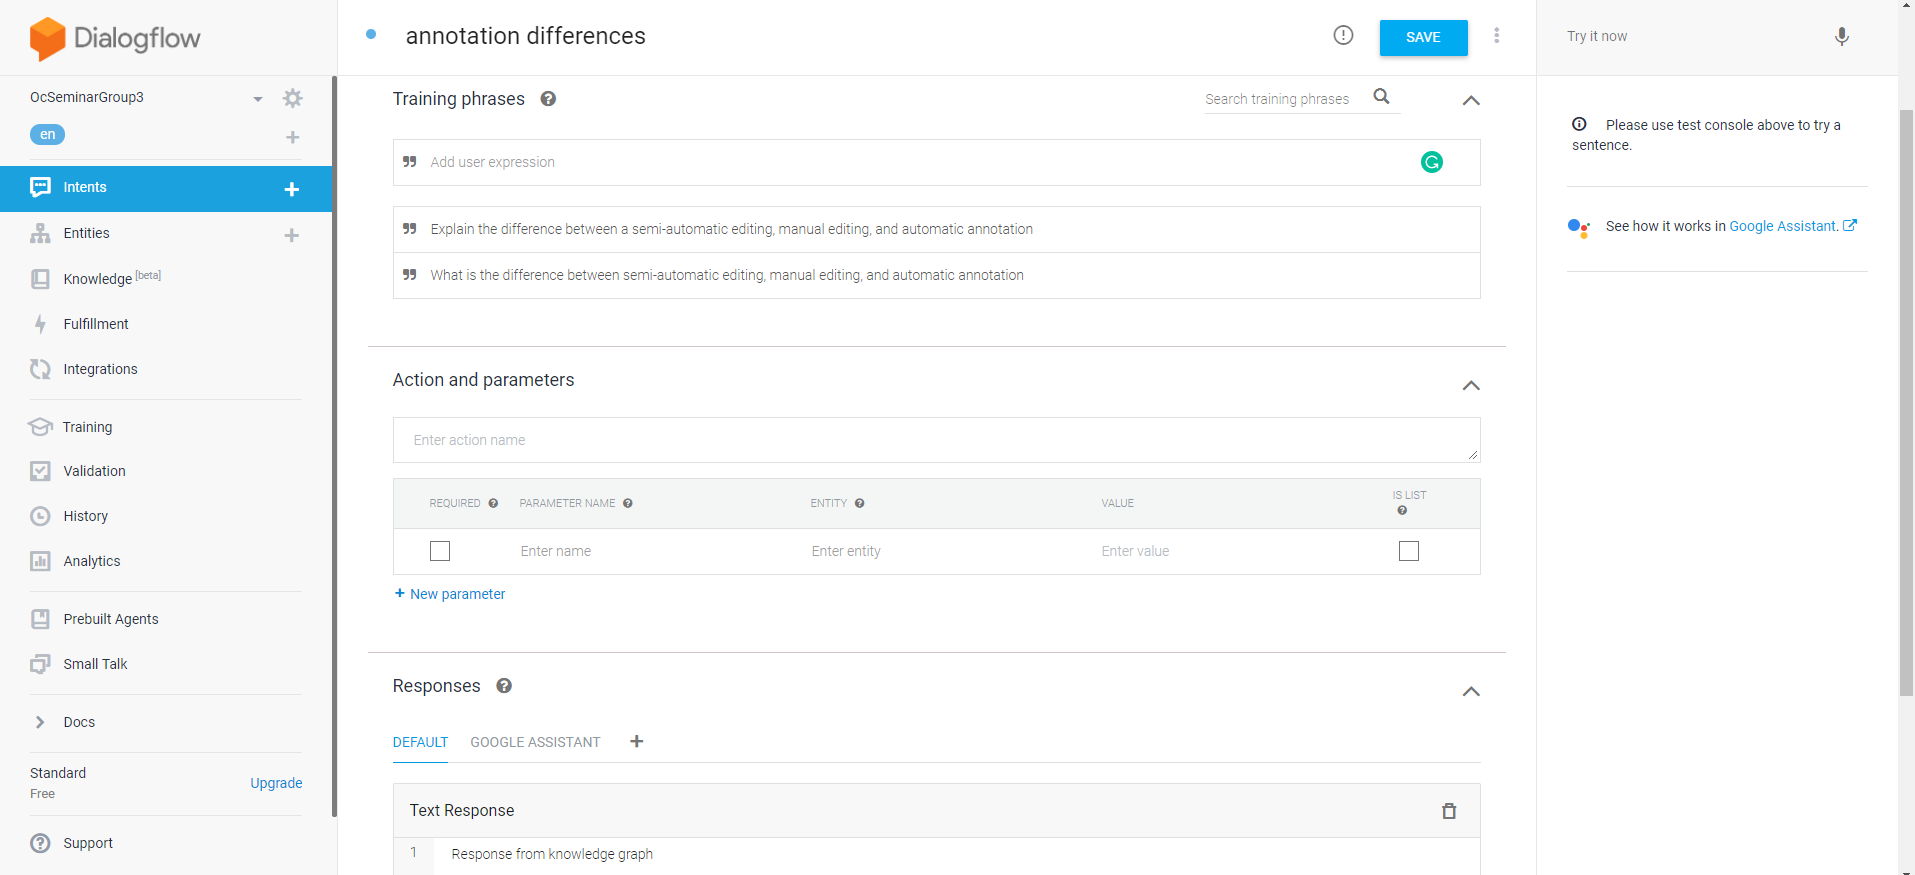
\includegraphics[width=\textwidth]{pictures/intents.png}

\end{center}
\end{frame}

%------------------------------------------------

\subsection{Entities}

\begin{frame}
\frametitle{Entities}
\begin{center}
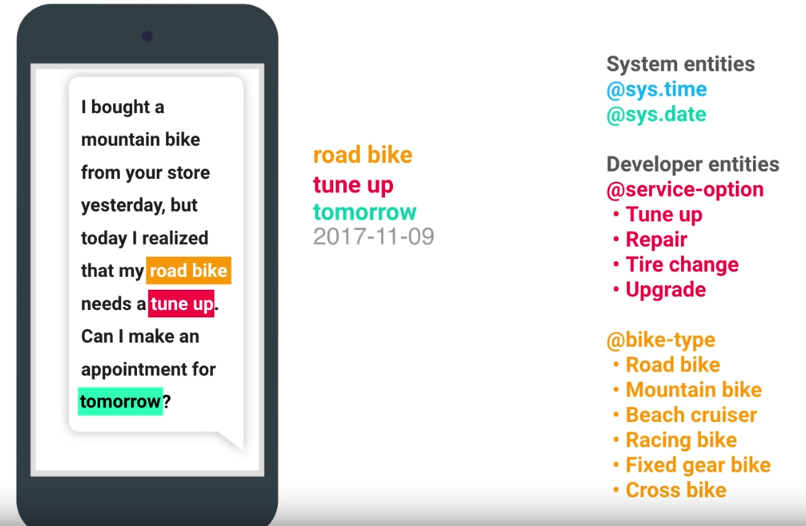
\includegraphics[width=0.8\textwidth]{pictures/entities2.png}
\end{center}
\end{frame}

\begin{frame}
\frametitle{Entities cont'd}
\begin{center}
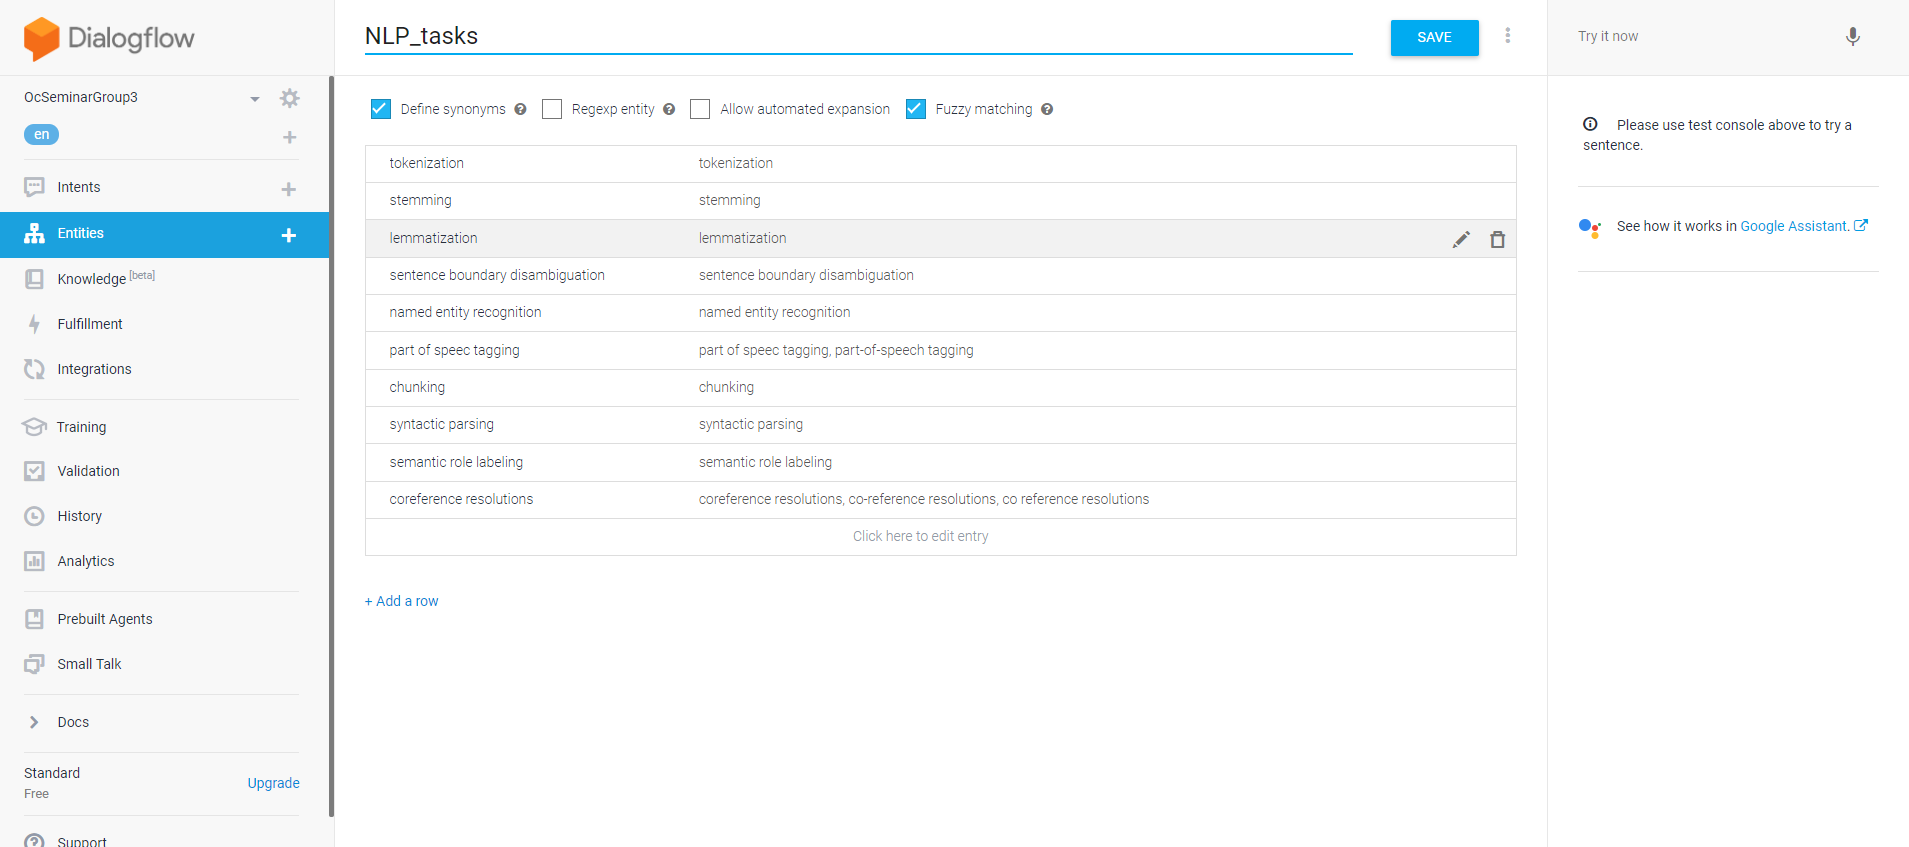
\includegraphics[width=\textwidth]{pictures/entities.png}
\end{center}
\end{frame}

%------------------------------------------------

\subsection{Knowledge Base}

\begin{frame}
\frametitle{Knowledge Base}
\begin{block}{Problem}
We need to somehow add the Knowledge Base from Group 1 into our skill.
\end{block}


\begin{block}{Solution}
There is a Knowledge Base feature which is already implemented in Dialogflow. However here we only can use documents like texts or csv files or pdfs. So we are not exactly sure how to handle this at the moment.
\end{block}

\end{frame}

%------------------------------------------------

\subsection{Fulfillment}

\begin{frame}
\frametitle{Fulfillment}
\begin{center}
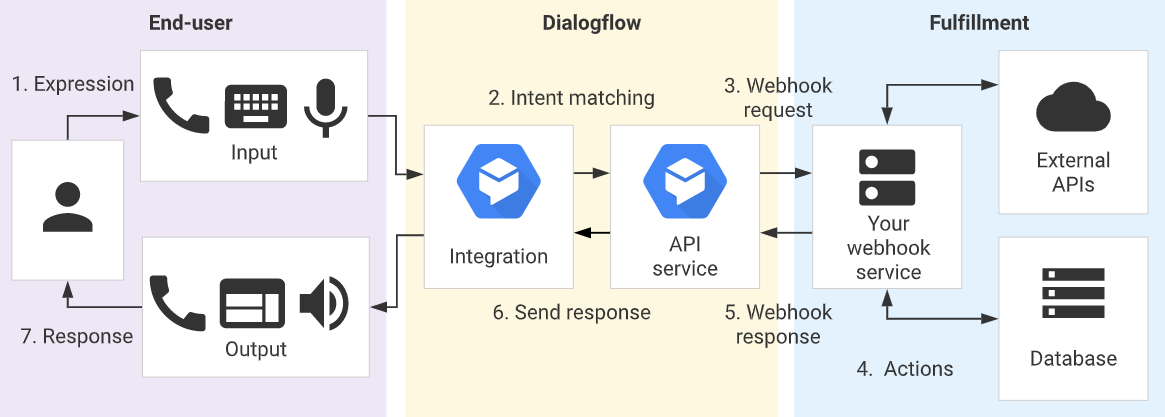
\includegraphics[width=\textwidth]{pictures/fulfillment_flow.png} 
\end{center}
\end{frame}

%------------------------------------------------

\subsection{Connecting to our GraphDB}

\begin{frame}
\frametitle{Connecting to our GraphDB}
\begin{block}{Problem}
Dialogflow doesn't allow direct connection to a database like Mycroft etc.
\end{block}


\begin{block}{Solution}
\begin{itemize}
\item Dialogflow sends a webhook request message that contains information about the matched intent, the action, the parameters, and the response defined for the intent.
\item Our service then performs the needed database query.
\item Our service sends back a webhook response containing the response to be sent to the end-user.
\end{itemize}
\end{block}

\end{frame}

%------------------------------------------------

\subsection{Webhook Service}

\begin{frame}
\frametitle{Webhook Service}
\begin{block}{Features}
\begin{itemize}
\item Supports Mutual TLS authentication.
\item Body of request and response is a simple JSON object.
\item Supports contexts and sessions, follow-up events and custom payloads.
\item Response can be a text, card, event or a Google Assistant response.
\end{itemize}
\end{block}


\begin{block}{Limitations}
\begin{itemize}
\item Response must occur within 10 seconds for Google Assistant applications or 5 seconds for other application, else it will timeout. 
\item The response must be less than or equal to 64 KiB in size.
\end{itemize}
\end{block}

\end{frame}

%------------------------------------------------

\section{Compatible Devices}

\begin{frame}
\frametitle{Compatible Devices}
\begin{center}
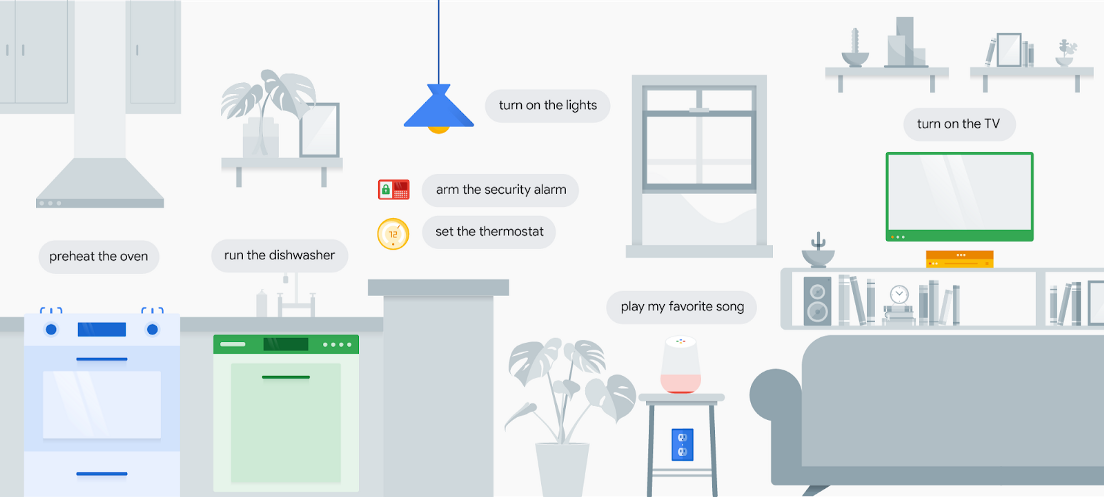
\includegraphics[scale=0.30]{pictures/smart_home.png} 
\end{center}
\end{frame}

\begin{frame}
\frametitle{Compatible Devices cont'd}
\begin{block}{Google Smart Home}
\begin{itemize}
\item Google \& IoT Devices
\begin{itemize}
\item Accessing to third-party IoT devices through Google Assistant
\item Use \textit{Actions} as Natural Language Understanding
\item Communication between \textit{Google Assistant} and IoT devices handled via cloud services.
\item \textit{Home Graph} to store information of connected devices
\end{itemize}
\end{itemize}
\end{block}
\end{frame}

\begin{frame}
\frametitle{Device Types \& Traits}
\begin{center}
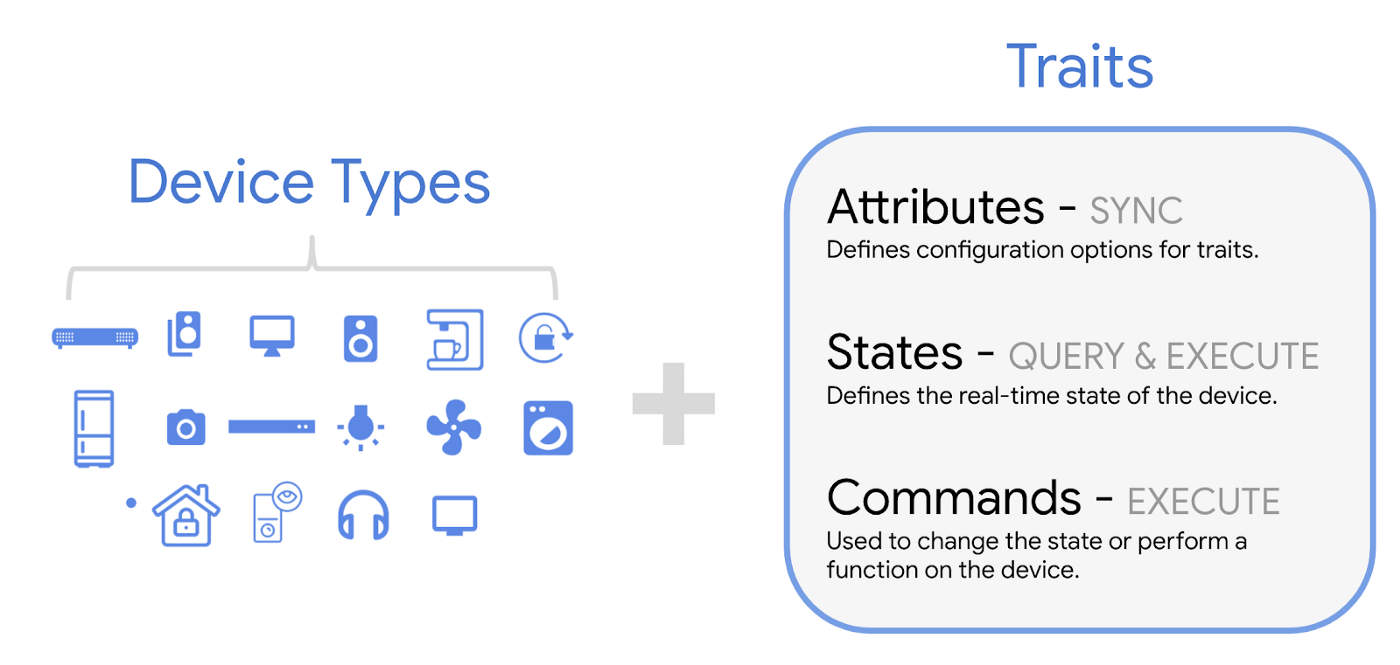
\includegraphics[scale=0.2]{pictures/state_commands.png} 
\end{center}
\begin{itemize}
\item Various device types ( air purifier to yogurt maker )
\item Capabilities of a device $\Rightarrow$ traits
\end{itemize}
\end{frame}

\begin{frame}
\frametitle{Sample Trait Schema}
\begin{center}
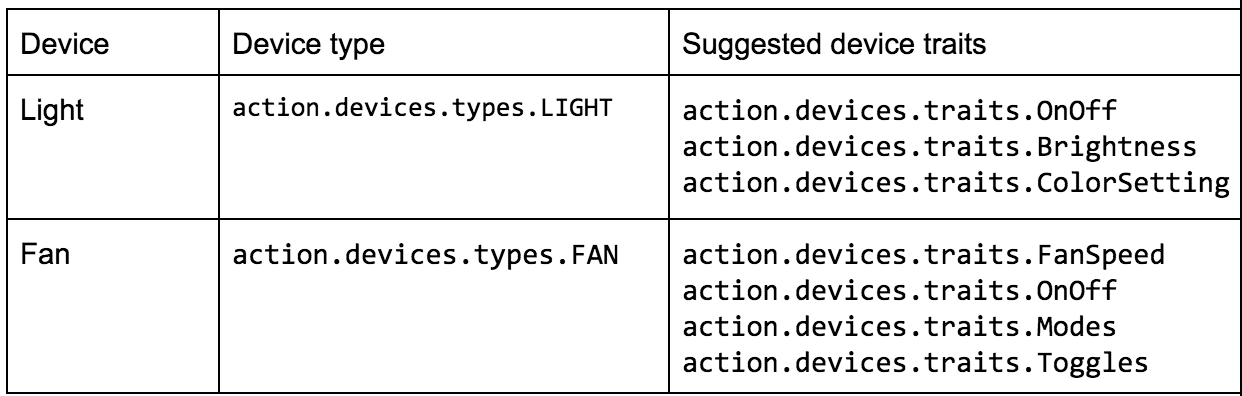
\includegraphics[scale=0.25]{pictures/types_and_traits.png} 
\end{center}
\end{frame}

\begin{frame}
\frametitle{Life Cycle}
\begin{center}
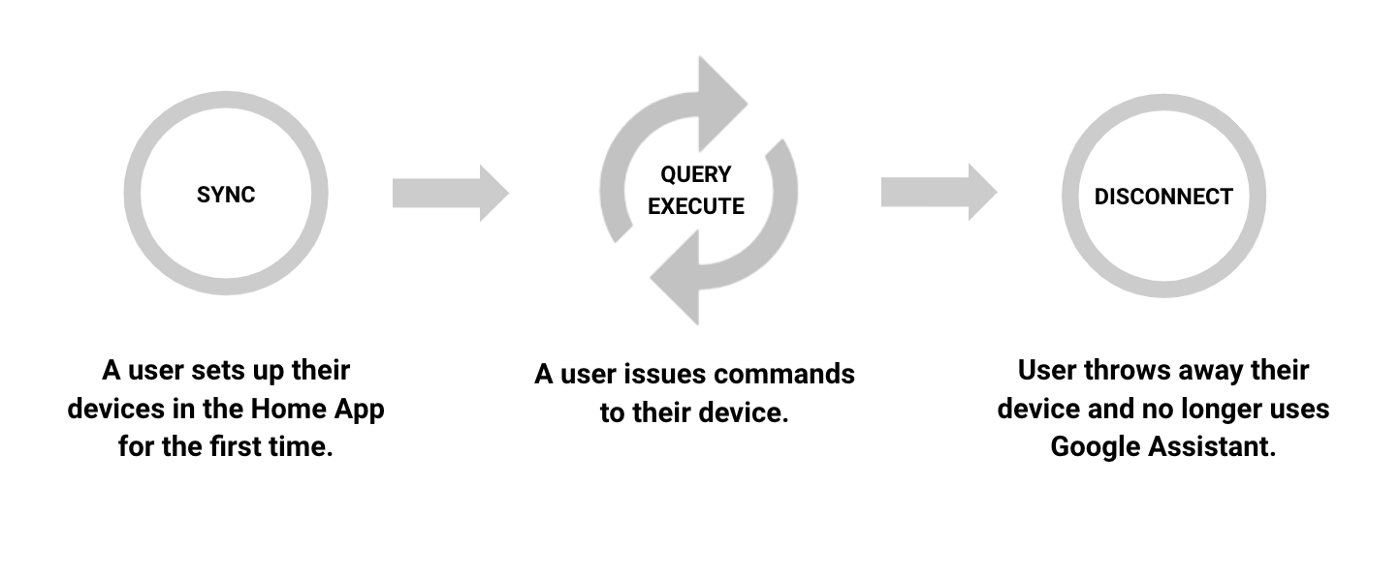
\includegraphics[scale=0.22]{pictures/cycle.png}
\end{center}
\end{frame}

\begin{frame}
\frametitle{Communication}
\begin{center}
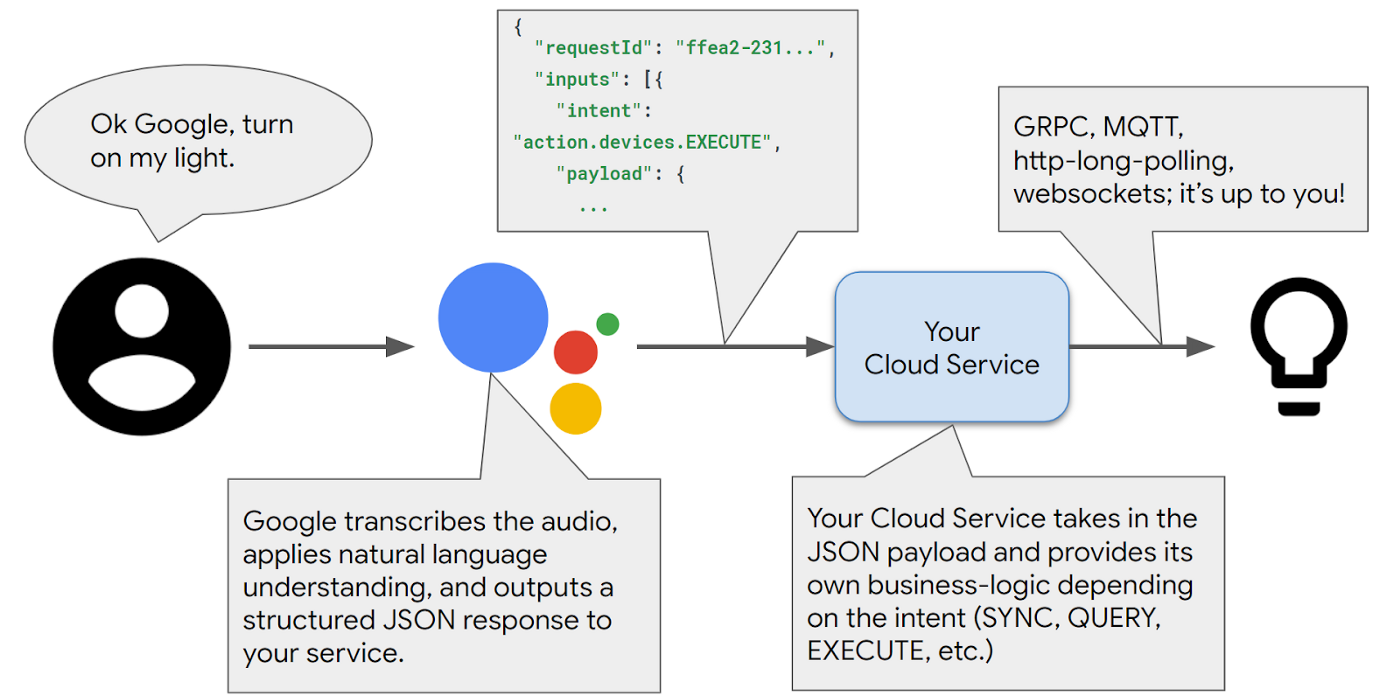
\includegraphics[scale=0.22]{pictures/communication_btw.png}
\end{center}
\end{frame}

%------------------------------------------------

\section{Live Demo}

\begin{frame}
\frametitle{Live Demo}
\begin{center}
{\fontsize{30}{40}\selectfont Live Demo}
\end{center}
\end{frame}

%------------------------------------------------

\begin{frame}
\begin{center}
{\fontsize{30}{40}\selectfont Thank you for your attention!}
\end{center}
\end{frame}

%------------------------------------------------

\end{document} 
